\documentclass[12pt]{report}

% \usepackage{polski}
\usepackage[polish]{babel}
\usepackage[utf8]{inputenc}
\usepackage{mathptmx}
\usepackage{graphicx} % do wstawiania png, pdf
\usepackage{caption} % zmniejszenie rozmiaru podpisów
\usepackage{air-title-page}
\usepackage{diagbox} % przekątne w komórkach
\usepackage{multirow} 
\usepackage{titlesec} % modyfikacja tytułów
\usepackage{hyperref} % łącza do referencji i w spisach
\usepackage[backend=biber,style=numeric,sorting=none]{biblatex}
\usepackage{rotating} % obracanie
\usepackage{longtable} %tabele na kilku stronach
\usepackage{float}
\usepackage{booktabs} %for \specialrule command
\usepackage{array}
\usepackage{algpseudocode}
\usepackage[shortlabels]{enumitem} % łatwa modyfikacja wyliczenia
\usepackage[titles]{tocloft}
\usepackage[T1]{fontenc} % font times new roman
\usepackage{mathptmx}

%==========Parametry strony tytułowej==========
\uczelniaNazwa{POLITECHNIKA WARSZAWSKA}
\uczelniaLogo{img/pw.pdf}
\wydzial{Wydział Mechatroniki}
\instytut{Instytut Automatyki i Robotyki}
\rok{2017}
\promotor{dr hab. inż. Michał Bartyś}
\temat{Projekt systemu monitorującego zużycie mediów komunalnych}
\autor{Krystian Kałużny}
\miasto{Warszawa}
%==============================================

%====================Wygląd====================
% \setmainfont{Liberation Serif}  %% Najbliższa Times New Roman http://askubuntu.com/questions/346552/closest-alternative-to-times-new-roman
% \setmainfont{Times New Roman}
\linespread{1.3} % odległość między liniami 1.5cm
\setlength{\parindent}{4em} %wielkość wcięcia akapitów

%  Głębokości sekcji
%  \part = -1
%  \chapter = 0
%  \section = 1
%  \subsection = 2
%  \subsubsection = 3
%  \paragraph = 4
%  \subparagraph = 5

\setcounter{secnumdepth}{3} % numeruj do subsubsekcji
\setcounter{tocdepth}{3} % dołącz subsubsekcję do table of content

\titleformat{\chapter}[display]{\normalfont\huge\bfseries}{\chaptertitlename\ \thechapter}{20pt}{\Huge}
\titlespacing*{\chapter}{0pt}{-50pt}{30pt} %{wcięcie poziome}{odstęp od początku strony do "Rozdział X"} {odstęp od tytułu rozdziału do zawartości}
\titleformat{\paragraph}{\normalfont\normalsize\bfseries}{\theparagraph}{1em}{}
\titlespacing*{\paragraph}{0pt}{3.25ex plus 1ex minus .2ex}{1.5ex plus .2ex}

%A4, jednostronny, marginesy
%headsep=1.2cm, headheight=16pt
\usepackage[a4paper, inner=2.5cm, outer=2.0cm, top=2.5cm, bottom=2.5cm]{geometry}
%==============================================
%======================Inne====================
\newcolumntype{C}[1]{>{\centering\let\newline\\\arraybackslash\hspace{0pt}}m{#1}} % definicja typu kolumny: wycentrowanego o określonej szerokości
\newcolumntype{[}[1]{@{\vrule width #1 \hskip\tabcolsep}} % separator kolumn o dowolnej grubości - dla pierwszej kolumny
\newcolumntype{!}[1]{@{\hskip\tabcolsep\vrule width #1 \hskip\tabcolsep}} % separator kolumn o dowolnej grubości - dla środkowych kolumn 
\newcolumntype{]}[1]{@{\hskip\tabcolsep\vrule width #1}}  % separator kolumn o dowolnej grubości - dla ostatniej kolumny
%parametry booktabs
\belowrulesep=0pt
\aboverulesep=0pt

%odstępy w toc
\setlength{\cftbeforechapskip}{.1ex}
\setlength{\cftbeforesecskip}{-.5ex}

% mniejsza czcionka w tabelach
\makeatletter
\renewenvironment{table}{%
	\renewcommand* {\@floatboxreset}{%
		\reset@font\@setminipage}
		\small\@float{table}}
   {\end@float}
\makeatother

% zmniejszenie rozmiaru podpisów
\captionsetup{font=small}
%==============================================

\addbibresource{bibliography.bib}
\begin{document}
	% \nocite{*} %wyświetlenie wszystkich wpisów z bibligrafi (nawet tych nieużywanych)
\pagenumbering{gobble}% Remove page numbers (and reset to 1)

\airtitlepage %własna strona tytułowa

\thispagestyle{empty}

\vspace*{2cm}

\begin{center}
	\textbf{Życiorys}
\end{center}
\begin{figure}[ht] %pływające otoczenie, h - zacznij tam gdzie zaczyna się tekst, t - umieść na górze strony
	\begin{minipage}[b]{0.35\textwidth} %minipage - niezależny alias strony
		\centering
		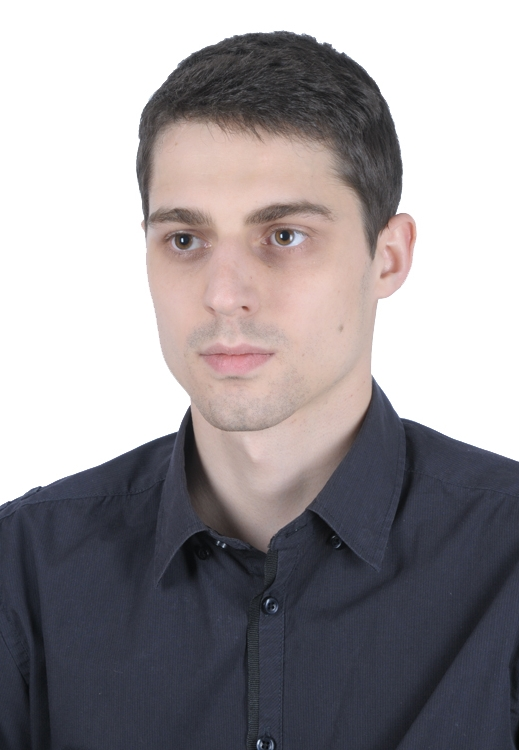
\includegraphics[width=\textwidth]{img/me-cv.jpg}
	\end{minipage}
	\hspace{0.5cm}
	\begin{minipage}[b]{0.6\textwidth}
		\begin{flushleft}
		Ireneusz Szulc
		
		{\it Kierunek:} Automatyka i Robotyka
		
		{\it Specjalność: } Informatyka przemysłowa
		
		{\it Urodzony:} 21. marca 1993~r. w Lublinie.
		
		{\it Numer indeksu:} 251001
		
		\end{flushleft}
	\end{minipage}
\end{figure}

Urodziłem się w Bździszewie.
W 2009 roku ukończyłem Gimnazjum w Woli Uhruskiej.
Następnie uczęszczałem do I Liceum Ogólnokształcącego im. Stefana Czarnieckiego w Chełmie.
W 2012 zdawałem maturę na poziomie rozszerzonym z matematyki i fizyki. 
Po maturze kontynuowałem naukę na Politechnice Warszawskiej na Wydziale Mechatroniki na kierunku Automatyka i Robotyka. 

\vspace{2cm}

\begin{flushright}
%bez wcięcia
	\noindent...................................
\end{flushright}

\newgeometry{tmargin=0cm, bmargin=0cm, lmargin=0cm, rmargin=0cm}
\begin{figure}[t]
	\centering
	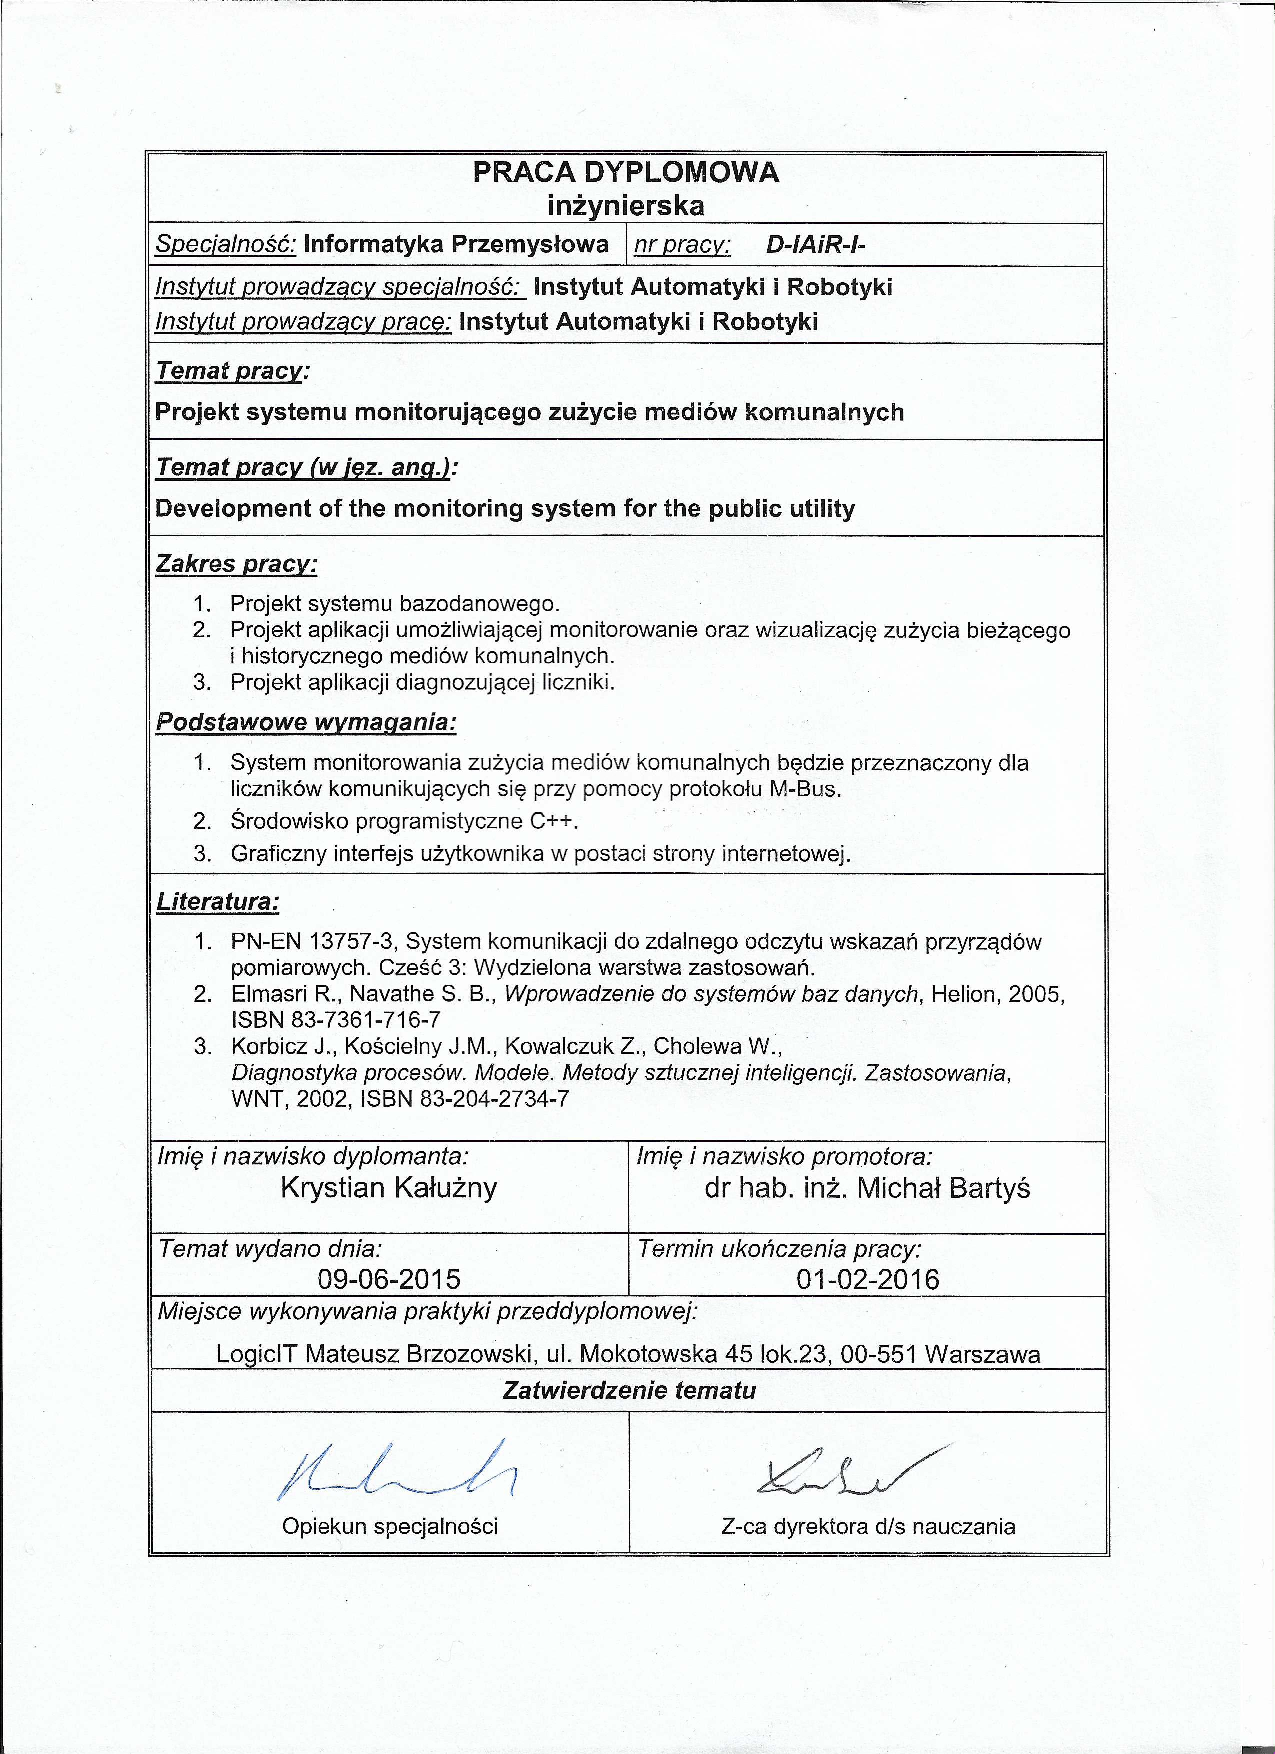
\includegraphics[scale=1.0]{img/karta-tematu.pdf}
	\label{fig:karta_tematu}
\end{figure}
\restoregeometry

\noindent {\Large\textbf{Streszczenie}}

TODO: Streszczenie PL

\pagebreak

\noindent {\Large\textbf{Abstract}}

TODO: Abstract

Path planning for a group of mobile robots

\pagebreak

\tableofcontents

\pagebreak
\pagenumbering{arabic}% Arabic page numbers (and reset to 1)

% Rozdział 1: Pierdolenie o Szopenie
\chapter{Wprowadzenie} % (fold)
\label{cha:wprowadzenie}

TODO: Celem pracy jest pierdolenie o Szopenie oraz pierdolenie kotka za pomocą młotka.


$TODO$ Konspekt:

Cel pracy
	system dla szpitali, dostarczania dokumentów, paczek
Założenia
	Aplikacja powinna umożliwiać symulację ruchu robotów oraz definiowanie położenia przeszkód przez użytkownika
	Planowanie tras dotyczy robotów holonomicznych
Wstęp teoretyczny
	algorytm A*
	systemy wilorobotowe
	wyznaczanie bezkolizyjnych tras
	słowniczek:
		robot holonomiczny
	tłumaczenie prezentacji o priorytetyzacji
	tłumaczenie innych prac angielskich :)
Projekt algorytmu wyznaczania trajektorii dla pojedynczego robota
	algorytm A* - opis algorytmu, implementacja, znajdzie rozwiązanie jeśli istnieje, nie jest optymalny, modyfikacja o omijanie ścian, ale z możliwością ruchu ukośnego
	potential field - słabe, problem minimów lokalnych bardzo mocny
Algorytm detekcji i zapobiegania kolizjom między robotami
	wyznaczanie globalnie optymalnego rozwiazania (centralnie) - jaki algorytm?
	lokalne podejmowanie decyzji na podstawie zasad (ruch drogowy)
	priorytetyzacja i wyznaczanie dróg:
		A star time-space - algorytm ?
		Path coordination - algorytm ?
		metoda wyznaczania priorytetów:
			metoda Monte Carlo?
			metoda największego spadku?
Implementacja oprogramowania symulacyjnego
	wykrzystane technologie - czyli co tygryski lubią najbardziej
	Java, Spring, Spring Boot, JavaFX, IntelliJ Ultimate, wzorce projektowe, klasy Immutable
	kluczowe algorytmy: symulacja ruchu robota w A* - schemat blokowy
	umożliwienie tworzenia mapki, definiowanie położenia przeszkód przez usera
	diagram klas?
	screeny
Przeprowadzenie testów symulacyjnych
	dużo testów
	dużo screenów

	
\chapter{Implementacja}
\label{cha:implementacja}

\section{Wymagania}

Postawiono następujące wymagania funkcjonalne:
\begin{itemize}
	\item pierdolenie o Szopenie
	\item pierdolenie kotka za pomocą młotka
\end{itemize}


\chapter{Testy aplikacji} % (fold)
\label{cha:testy}

Nie starczyło czasu na testy.


\chapter{Podsumowanie} % (fold)
\label{cha:podsumowanie}

$TODO$
Latex formatting cheatsheet:
\begin{itemize}
	\item \textit{echo}
	\item $ 255.255.255.255 $
	\item równania
	\item obrazki
	\item tabelki
	\item chaptery
	\item section, subsection
	\item linki do bibliografii
	\item linki do obrazków
\end{itemize}



\listoffigures

\listoftables

\printbibliography

% %\appendix
\chapter*{Spis załączników}

Na załączonej do pracy płycie CD znajdują się następujące treści:
\begin{itemize}
	\item Niniejsza praca w formacie PDF -- plik\\ \textit{Praca/Praca\_Magisterska\_Ireneusz\_Szulc.pdf}.

	\item Archiwum zawierające kody źródłowe programu symulacyjnego -- plik\\ \textit{Kody\_źródłowe/apliakcja-symulacja.zip}

\end{itemize}

\end{document}
